%!TEX program = xelatex
% Importar configuración
\input{_preamble.tex}

\title{Generación de representaciones alternativas de datos mediante técnicas no supervisadas de Deep Learning}
\date{12 de julio de 2018}
\author{Francisco David Charte Luque\\\scriptsize Tutores: \textbf{Francisco Herrera} y \textbf{Francisco Charte}\\}
\institute{\myserif\includegraphics[width=0.3\textwidth]{ugr-logo.eps} \flushright\vspace{-1.05cm}Máster en Ciencia de Datos e Ingeniería de Computadores}

\begin{document}
\begin{frame}[plain]
\maketitle
\end{frame}

\section{Introducción}
%% \begin{frame}{Trabajo previo}
%%   \begin{theorem}
%%     \label{th:dim-curse}
%% Sea \(\{F_{m}\}_{m\in\mathbb N}\) una sucesión de distribuciones de
%% probabilidad, \(n\in \mathbb N\) y \(p\in\mathbb R^+\) fijos. Para cada
%% \(m\in\mathbb N\) sean \(X_{m1},\dots,X_{mn}\sim F_m\) muestras independientes
%% e idénticamente distribuidas. Supongamos que tenemos una función
%% \(d_m:\mathrm{Dom}(F_m)\rightarrow \mathbb R^+_0\) y llamamos
%% \begin{align*}
%%   \mathrm{DMIN}_{m}&=\operatorname{min}\{d_m(X_{mi}):i=1,\dots,n\},\\
%%   \mathrm{DMAX}_{m}&=\operatorname{max}\{d_m(X_{mi}):i=1,\dots,n\}.
%% \end{align*}
%% Entonces, si
%% \(\operatorname{lim}_{m\rightarrow +\infty}\operatorname{Var}\left[\frac{d_m(X_{m1})^p}{E[d_m(X_{m1})^p]}\right]=0\)
%% se tiene que, para cada \(\varepsilon > 0\),
%% \[\operatorname{lim}_{m\rightarrow +\infty}\operatorname{Pr}\left[{\mathrm{DMAX}_m\leq (1+\varepsilon) \mathrm{DMIN}_m}\right]=1.\]
%%   \end{theorem}

%% \end{frame}

\begin{frame}{Introducción}

\begin{itemize}
\item Redes neuronales artificiales: basadas en el \alert{perceptrón} (1949), cálculo de gradientes con \alert{\textit{backpropagation}} (1896).
\item Aprendizaje no supervisado (sin etiquetas), en concreto \alert{fusión de características}.
\item Arquitectura existente: el \alert{autoencoder}
\end{itemize}

\begin{figure}[h!]
\centering
\includegraphics[width=0.2\linewidth]{../inffus/ShallowUndercomplete.pdf}\quad
\includegraphics[width=0.2\linewidth]{../inffus/ShallowOvercomplete.pdf} \quad
\includegraphics[width=0.2\linewidth]{../inffus/DeepUndercomplete.pdf} \quad
\includegraphics[width=0.2\linewidth]{../inffus/DeepOvercomplete.pdf} 
\end{figure}


\end{frame}


\section{Teoría: autoencoders}
\subsection*{}

\frame{
\begin{block}{\centering A practical tutorial on autoencoders for nonlinear feature fusion: Taxonomy, models, software and guidelines}
\centering
\small D. Charte\quad F. Charte\quad S. García\quad M.J. del Jesus\quad F. Herrera\\
Information Fusion 44 (2018)
\end{block}

Los \alert{autoencoders} son una familia creciente de herramientas para fusión de características. Contenidos del paper:
\begin{itemize}
\item Proponemos una taxonomía de las variantes y las detallamos
\item Los comparamos con otras técnicas
\item Estudiamos las aplicaciones
\item Proveemos pautas de diseño
\item Enumeramos el software disponible
\end{itemize}
}

\begin{frame}{Taxonomía}

\begin{figure}[htp!]
	\centering
	\resizebox {\textwidth} {!} {
		
		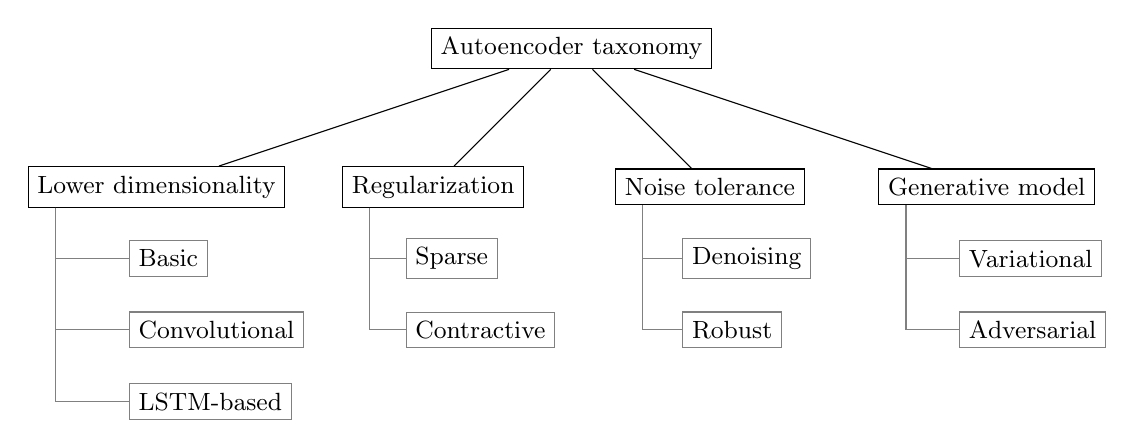
\begin{tikzpicture}[
		font=\small,
		every node/.style = {shape=rectangle,
			draw, align=center},
		level 1/.style={sibling distance=10em},
		level 2/.style={grow=down, anchor=west, draw=gray, xshift=-1em,
			edge from parent path={([xshift=1em]\tikzparentnode.south west) |- (\tikzchildnode.west)}},
		level distance=5em,
		first/.style={level distance=6ex,xshift=-1em},
		second/.style={level distance=12ex,xshift=-1em},
		third/.style={level distance=18ex,xshift=-1em},
		],
		
		\node {Autoencoder taxonomy}
		child { node {Lower dimensionality}
			child[first]  { node {Basic} }
			child[second] { node {Convolutional} }
			child[third]  { node {LSTM-based} }
		}
		child { node {Regularization}
			child[first]  { node {Sparse} }
			child[second] { node {Contractive} }
		}
		child { node {Noise tolerance}
			child[first]  { node {Denoising} }
			child[second] { node {Robust} }
		}
		child { node {Generative model}
			child[first]  { node {Variational} }
			child[second] { node {Adversarial} }
		};
		\end{tikzpicture}
	}
%	\caption{Taxonomy: most popular autoencoders classified according to the charasteristics they induce in their encodings}
	\label{fig:autoencoder-taxonomy}
\end{figure}
\end{frame}

\begin{frame}{Autoencoder básico}
\begin{columns}[t]
\column{0.5\textwidth}
\header{Estructura}

\emph{encoder}-\emph{decoder}:
\begin{align*}
  y&=f(x)=s_1(W^{(1)}x+b^{(1)}),\\
  r&=g(y)=s_2(W^{(2)}y+b^{(2)})
\end{align*}

\vspace{.1cm}
\header{Función objetivo}
\vspace{-.5cm}
\begin{equation*}
\mathcal J(W,b;S)= \sum_{x \in S} \mathcal L(x, (g\circ f)(x))
\end{equation*}


\vspace{.1cm}
\header{Stacking}

Proceso por el cual se entrena \alert{capa a capa} de forma voraz. 

\column{0.5\textwidth}
\header{Entrenamiento}

Algoritmos basados en descenso del gradiente estocástico:
\begin{itemize}
\item AdaGrad
\item RMSProp
\item Adam
\item ...
\end{itemize}

Cómputo de gradientes mediante \emph{backpropagation}.


\end{columns}
\end{frame}

\begin{frame}{Autoencoders con regularización}
\begin{columns}[t]
\column{0.5\textwidth}
\header{Sparse}

Objetivo: minimizar activaciones en capa de codificación.

Regularización: \[
  \Omega_{\mathrm{SAE}}(W,b;S)=\sum_{i=1}^c \mathrm{KL}(\rho\Vert \hat\rho_i)
\]

\begin{center}
\includegraphics[width=0.6\columnwidth]{../inffus/kldivergence.pdf} 
\end{center}


\column{0.5\textwidth}
\header{Contractive}

Objetivo: menor sensibilidad a pequeños cambios en las entradas.

Regularización:
\[
\Omega_{\mathrm{CAE}}(W,b;S) = \sum_{x\in S}\left\lVert J_f(x) \right\rVert_F^2~.
\]


\end{columns}
\end{frame}

\begin{frame}{Autoencoders resistentes a ruido}
\begin{columns}[t]
\column{0.5\textwidth}
\header{Denoising}

Entrenamiento con datos corruptos/ruidosos.

\begin{center}
\includegraphics[width=0.9\columnwidth]{../inffus/Denoising.pdf}
\end{center}

\column{0.5\textwidth}
\header{Robust}

Función objetivo: correntropía
\begin{align*}
  \mathcal L_{\mathrm{MCC}}(u, v)&=-\sum_{k=1}^d\mathcal K_{\sigma}(u_k-v_k),\\
  \mathcal K_{\sigma}(\alpha)&=\frac{1}{\sqrt{2\pi}\sigma}\exp\left(-\frac{\alpha^2}{2\sigma^2}\right)
  \end{align*}

Más resistente a ruido no Gaussiano (p.ej. Cauchy)

\end{columns}
\end{frame}

\begin{frame}{Otros}
\begin{columns}[t]
\column{0.5\textwidth}
\header{Dominio específico}

\begin{itemize}
\item Convolutional: procesamiento de estructuras 2D, 3D
\item LSTM-based: procesamiento de secuencias
\end{itemize}

\column{0.5\textwidth}
\header{Modelo generativo}

\begin{itemize}
\item Variational
\item Adversarial
\end{itemize}

Permiten generar nuevas instancias.

\end{columns}
\end{frame}


\begin{frame}{Comparación y aplicaciones}
\begin{columns}[t]
\column{0.5\textwidth}
\header{Otras técnicas}

\begin{itemize}
\item PCA = AE lineal + MSE
\includegraphics[width=0.9\columnwidth,trim={14em 16.5em 12em 1.5em},clip]{../inffus/pca-36.pdf}\\\vspace{-.1cm}
  \includegraphics[width=0.9\columnwidth,trim={14em 2em 12em 17em},clip]{../inffus/pca-36.pdf}\\\vspace{-.1cm}
  \includegraphics[width=0.9\columnwidth,trim={14em 2em 12em 17em},clip]{../inffus/basic-36-linear-rmsprop-mse.pdf}

\item AE no lineal es más general que Kernel PCA
\item CAE tiene aspectos similares con Isomap/LLE
\item RBM es una alternativa para inicialización capa-a-capa
\end{itemize}


\column{0.5\textwidth}
\header{Aplicaciones}

\begin{itemize}
\item Clasificación
\item Compresión de datos
\item Detección de anomalías
\item Hashing
\item Visualización
\item Reconstrucción
\item Otras
\end{itemize}

\end{columns}
\end{frame}

\begin{frame}{Diseño de autoencoders}
\begin{columns}[t]
\column{0.5\textwidth}
\header{Pautas}

\begin{itemize}
\item Arquitectura: ¿longitud de codificación?
\item Activaciones y función objetivo: sigmoide con XENT y no mayoradas con MSE
\item Regularizaciones: \emph{weight decay}?, \emph{sparsity}?
\end{itemize}

\column{0.5\textwidth}
\header{Software}

\begin{itemize}
\item Tensorflow
\item Caffe
\item Torch
\item MXNet
\item \alert{Keras}
\end{itemize}

Paquetes con AEs: SAENET, Autoencoder, H2O, yadlt

\end{columns}
\end{frame}


%% \begin{frame}[fragile]{Otra diapositiva}
%% \begin{verbatim}
%% $ git clone git@github.com:libreim/templates
%% $ cd templates
%% \end{verbatim}
%% \end{frame}


\section{Práctica: paquete Ruta}\subsection*{}

\begin{frame}[fragile]{Descripción}

\begin{columns}[c]
\column{.5\textwidth}

\includegraphics[width=0.2\columnwidth]{imgs/ruta_logo64}

Paquete de R implementado sobre \alert{Keras + Tensorflow}. Publicado en CRAN:

\small
\begin{verbatim}
install.packages("ruta")
\end{verbatim}
\normalsize

Documentación: \href{https://ruta.software}{ruta.software}

\column{.5\textwidth}

\includegraphics[width=\columnwidth]{imgs/rutacran}

\flushright
\includegraphics[width=0.3\columnwidth,trim={0 7cm 0 0},clip]{imgs/gpl3}

\end{columns}

\end{frame}

\begin{frame}[fragile]{Uso}
\scriptsize
\begin{minted}[frame=lines]{R}
library(ruta)
library(purrr)

# Barajar y normalizar
x <- iris[, 1:4] %>% sample %>% as.matrix %>% scale
x_train <- x[1:100, ]
x_test <- x[101:150, ]

autoencoder(
  input() + dense(256) + dense(36, "tanh")
    + dense(256) + output("sigmoid"),
  loss = "mean_squared_error"
) %>%
  make_contractive(weight = 1e-4) %>%
  train(x_train, epochs = 40) %>%
  evaluate_mean_squared_error(x_test)
\end{minted}
\end{frame}

\begin{frame}{Funcionalidad implementada}

\begin{columns}[t]
\column{.4\textwidth}
\header{Autoencoders}

\begin{itemize}
\item básico
\item
sparse
\item
contractive
\item
denoising
\item
robust
\item
variational
\item
weight decay
\end{itemize}

\alert{Accesos a Keras} para más funcionalidad

\column{.6\textwidth}
\header{Tareas}
\begin{itemize}
\item entrenamiento
\item
codificación/decodificación
\item
reconstrucción
\item
evaluación
\item generación (variacional) 
\item
guardado de modelos
\item generación de ruido: Cauchy, gaussiano, unos, ceros, \emph{sal y pimienta}
\end{itemize}

\end{columns}
\end{frame}

\begin{frame}[fragile,shrink]{Ejemplos: AE robusto}

\scriptsize
\begin{minted}[frame=lines]{R}
network <- input() + dense(36, "elu") + output("sigmoid")
learner <- autoencoder_robust(network)
\end{minted}
\normalsize

\includegraphics[width=\columnwidth]{imgs/robust}

\includegraphics[width=\columnwidth]{imgs/robust_cauchy}

\end{frame}
\begin{frame}[fragile,shrink]{Ejemplos: AE variacional}
\scriptsize
\begin{minted}[frame=lines]{R}
network <-
  input() + dense(256, "elu") + variational_block(3, seed=42) +
  dense(256, "elu") + output("sigmoid")
learner <- autoencoder_variational(network,
  loss = "binary_crossentropy")
\end{minted}

\begin{columns}[c]

\column{.4\textwidth}
\includegraphics[width=\columnwidth]{imgs/variational}
\column{.6\textwidth}

\begin{minted}[frame=lines]{R}
model %>% generate(
  dimensions = c(1, 3),
  side = 5, fixed_values = 0.01
 )
\end{minted}
\end{columns}
\normalsize

\end{frame}

\section{Conclusiones}
\subsection*{}

\begin{frame}{Conclusiones}

\header{Trabajo futuro}
\begin{itemize}
\item AEs aplicados a aprendizaje \alert{no estándar} (multi-vista, multi-etiqueta, LDL...)
\item Construcción de \alert{ensembles}
\item Extensiones de Ruta: visualizaciones e interfaz web.


\end{itemize}

\header{Comentarios finales}
\begin{itemize}
\item Hemos estudiado y contextualizado los AEs
\item Se han implementado sobre Keras
\item Resultados: paper Q1 + software en CRAN
\end{itemize}

\end{frame}

\maketitle
\end{document}
